\section{Case Study}
\label{sec:grammars-and-metamodels:Case-Study}
We applied the surface language described in this chapter during a case study with an industrial partner.
As part of the Ideals project~\cite{Ideals2007}, we investigated a straightforward transformation from \UML models to formal models suited for performance analysis.
To ensure the straightforwardness of this transformation, detailed \UML models were required.
Initially, the behavior of the components of these models was described graphically using a combination of activity diagrams and state machine diagrams, where each state machine referred to a number of activities.
However, to reduce the amount of work required to produce these detailed models, we replaced some of the activity diagrams by equivalent descriptions of behavior expressed using our surface language.

For seven of the components of such a detailed \UML model, Table~\ref{tab:grammars-and-metamodels:ideals-table} shows the number of \Activities required to model part of their behavior.
Furthermore, the size of each of the corresponding activity diagrams is illustrated by means of the number of graphical elements contained by these diagrams.
In the rightmost column of the table, the number of statements of the corresponding textual specification is given.
On the left of Figure~\ref{fig:grammars-and-metamodels:ideals-example}, one of the \Activities of component~$A$ is shown, which consists of nine graphical elements.
On the right of the figure, an equivalent textual specification of this behavior is shown, expressed using our surface language.

\begin{table*}
\centering
\small
\begin{tabular}{|c|c|r|r|}
\hline
\rowcolor[gray]{.9}
                            & \textbf{Number of}   & \head{Number of graphical} & \head{Number of}\\
\rowcolor[gray]{.9}
\mr{-2}{\textbf{Component}} & \textbf{\Activities} & \head{elements}            & \head{statements}\\
\hline
A                           & 4                    & 9 + 6 + 5 + 8              & 3 + 1 + 1 + 2 \\
\hline
B                           & 2                    & 6 + 9                      & 1 + 2 \\
\hline
C                           & 2                    & 5 + 5                      & 1 + 1 \\
\hline
D                           & 4                    & 26 + 14 + 14 + 11          & 6 + 3 + 3 + 2 \\
\hline
E                           & 5                    & 17 + 11 + 15 + 16 + 17     & 4 + 2 + 3 + 4 + 4 \\
\hline
F                           & 5                    & 7 + 17 + 9 + 7 + 19        & 1 + 4 + 2 + 1 + 5 \\
\hline
G                           & 3                    & 6 + 6 + 6                  & 1 + 1 + 1 \\
\hline
\end{tabular}
\caption{Comparison of the size of graphical and textual specifications of behavior}
\label{tab:grammars-and-metamodels:ideals-table}
\end{table*}

Although most of the activity diagrams mentioned in Table~\ref{tab:grammars-and-metamodels:ideals-table} are small, such as the one in Figure~\ref{fig:grammars-and-metamodels:ideals-example}, creating them showed to be cumbersome and the amount of additional information they offer in comparison to the textual specifications is limited.
As mentioned above, each \UMLStateMachine is related to a number of \Activities.
Because of their conciseness, the textual equivalents of the \Activities could be incorporated directly into the diagrams of the related state machines, thus reducing the number of diagrams.

\begin{figure}
\centering
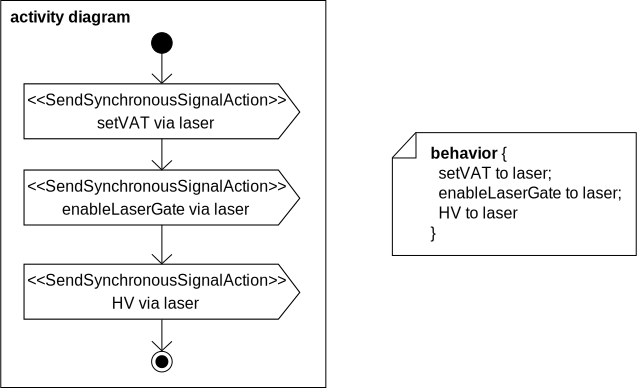
\includegraphics[scale=0.5]{grammars-and-metamodels/figs/ideals-example}
\caption{An Activity and its textual equivalent from the Ideals project}
\label{fig:grammars-and-metamodels:ideals-example}
\end{figure} 